\documentclass[a4paper]{article}

\usepackage[czech]{babel}
\usepackage[utf8]{inputenc}
\usepackage[T1]{fontenc}
\usepackage{tgpagella}

\usepackage[left=1.5cm, text={18cm, 26cm}, top=1.8cm]{geometry}

\usepackage{graphicx}
\usepackage{float}
\usepackage[usenames, dvipsnames]{xcolor}
\usepackage{pdflscape}

\usepackage[pdftex,
            pdfauthor={David Konecny, Martin Pech},
            pdftitle={Projekt},
            pdfsubject={IDS},
            pdfkeywords={IDS},
            pdfproducer={David Konecny, Martin Pech},
            pdfcreator={LaTeX on David's PC},
            unicode,
            hidelinks]{hyperref}
            

\newcommand{\logo} {
  \includegraphics[scale=0.8, keepaspectratio]{fig/logo.pdf}
}

\renewcommand*{\ttdefault}{lmtt}

\pdfminorversion=7


\begin{document}

  \begin{titlepage}
    \begin{center}
      \logo
      \\\vspace{\stretch{0.382}}
      {\Huge Databázové systémy -- Projekt, první část}\\\medskip
      {\LARGE Návrh struktury databáze}\\\medskip
      \vspace{\stretch{0.618}}
    \end{center}
  
    {\Large \today \hfill
      \begin{tabular}{l l}
	 	    David Konečný & (\texttt{xkonec83}) \\
	  	  Martin Pech   & (\texttt{xpechm00}) \\
	  \end{tabular}}
  \end{titlepage}

  \section{Úvod}
  \label{sec:intro}

    Tento projekt byl vypracován na základě projektu z~předmětu \textbf{IUS}, který byl hodnocen \textbf{21} body z~celkových 24 možných. Původním zadáním byl \textbf{Návrh informačního systému pro Fitness centrum}. Toto zadání bylo pro účely tohoto předměty modifikováno tak, aby výsledný návrh co nejlépe odpovídal reálnému světu a~reprezentoval smysluplnou databázi, na jejímž základě bude stát stabilní informační systém.
    
    \subsection{Zadání}
    \label{subsec:assignment}

      Uvažujme informační systém \emph{(dále jen \textbf{IS})}, pro který je potřeba navrhnout databázi. Požadavky na informačního systému jsou:
      
      \begin{itemize}
        \item Ukládat informace o~klientech a~klientských kartách
        \item Ukládat informace o~zaměstnancích
        \item Ukládat informace o~kvalifikacích některých pracovníků (\textit{instruktorů})
        \item Ukládat informace o~nabízených lekcích a~samotné lekce
        \item Ukládat informace o~registracích na nabízené lekce
      \end{itemize}

  \section{Model případů užití}
  \label{sec:use-case}

    \begin{figure}[H]
      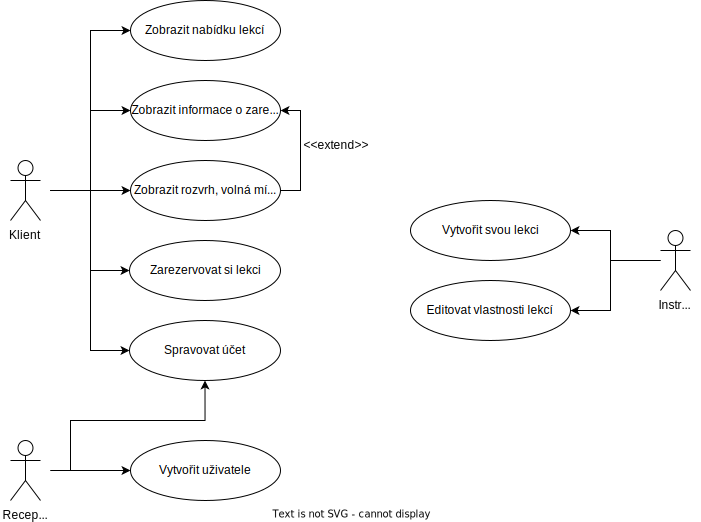
\includegraphics[scale=0.8, keepaspectratio]{fig/use_case.pdf}
    \end{figure}

  \newpage

  \section{ER diagram}
  \label{sec:er}

    \emph{ER Diagram} byl modelován na základě znalosti principů návrhu systému a~na základě požadavků (viz sekce~\ref{subsec:assignment}). Pro finální podobu byla zvolena \emph{Crow's Foot} notace. Ta umožňuje velice přesně znázornit vztahy, mezi jednotlivými entitami.
    
    \subsection{Entitní množiny}
    \label{subsec:entity}

      \begin{itemize}
        \item \textbf{Zaměstnanec} - Základní entitní, která ukládá informace o~zaměstnancích. Primárním klíčem je \texttt{ID\_zaměstnance}. Nabízela se možnost použít rodné číslo, avšak pro zamýšlené účely je ID příhodnější. Tato entita je dále zobecněním (\textit{generalizací}) entit \textbf{recepční} a~\textbf{instruktor}. Tyto entity rozdělují práva a~povinnosti dvou odlišných profesí.
        \item \textbf{Recepční} - Spravuje klientské účty (vytváří uživatele, přiděluje karty).
        \item \textbf{Instruktor} - Má vždy alespoň jednu kvalifikaci (\textit{specializaci}). Na základě toho vede učitý počet lekcí.
        \item \textbf{Kvalifikace} - Tabulka všech kvalifikací, které mohou trenéři mít.
        \item \textbf{Klient} - Další základní entita, která uchovává informace o~registrovaných klientech. Primárním klíčem je opět unikátní identifikátor klienta ve formě \texttt{ID\_klienta}. 
        \item \textbf{Klientská karta} - Na základě vytvoření uživatele je uživateli přidělena právě jedna členská karta, se kterou se může prokazovat. V~případě ztráty této karty je karta smazána ze systému a~uživateli je přídělena nová.
        \item \textbf{Rezervace} - Slabá entitní množina. Je závislá na množině \textbf{lekce}. Může je vytvářet uživatel.
        \item \textbf{Lekce} - Entitní množina uchovávající informace o~všech plánovaných (\textit{a některých proběhlých}) lekcích. Primárním klíčem je unikátní čislo lekce (\texttt{ID\_lekce}). Pokud neexistuje žádná lekce, není možné aby si klient vytvořil rezervaci. Slabá entitní množina \textbf{rezervace} je na ní tedy závislá. Pokud existuje, je možné aby se na ní registrovalo tolik klientů, kolik je kapacita lekce. Kapacita lekce se může lišit od kapacity místnosti. Tato entitní množina je zobecněním entit \textbf{Individuální lekce} a~\textbf{Skupinová lekce}. 
        \item \textbf{Skupinová lekce} - Skupinová lekce musí vždy probíhat v~nějaké místnosti.
        \item \textbf{Individuální lekce} - Nemá předem uvedenou místnost. Domluva o~plánu tréninku probíhá mezi instruktorem a~klientem přímo.
        \item \textbf{Místnost} - ukládá informace o~všech místnostech, ve kterých je možné pořádat lekce.
      \end{itemize}

    \begin{figure}[H]
      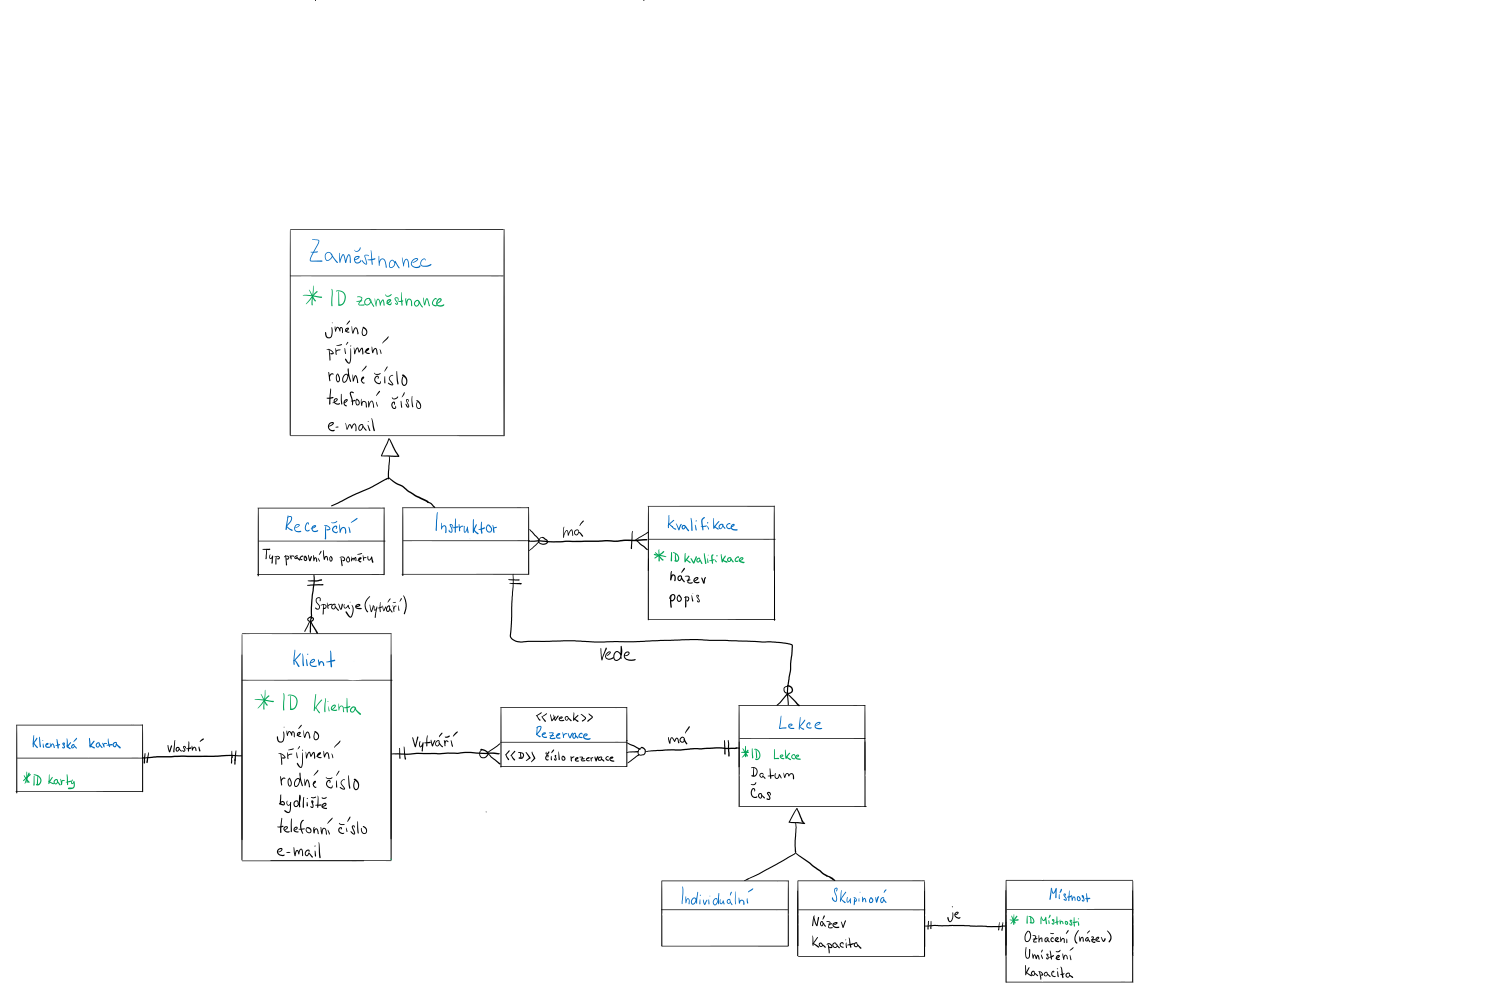
\includegraphics[scale=0.6, keepaspectratio]{fig/er.pdf}
    \end{figure}

  

\end{document}
